\section{Ejercicio 8}

En el ejercicio 8 se pide realizar una implementación del scheduler round robin, pero sin migración de procesos entre núcleos.
Para esto se agregaron nuevas estructuras a la clase SchedRR2:
\begin{itemize}
\item \textbf{colaReady}: Ahora es un vector de colas, las cuales van a almacenar los pid de las tareas que ultilicen el core correspondiente.
\item \textbf{cantTasks}: Indica la cantidad de tareas que tiene cada cpu (RUNNING + BLOCKED + READY).
\item \textbf{cpuTareasBloqueadas}: Es una cola de tuplas con un pid en la primera coordenada (proceso que hizo llamada bloqueante) y número de core en el cual estaba ejecutando.
\end{itemize}

Los métodos load, unblock y tick también cambian respecto del round robin con migración de procesos.

\begin{itemize}
\item \textbf{load(pid)}: Se encarga primero de buscar cual es el cpu con menor cantidad de tareas y, una vez encontrado, sumar uno a la cantTasks de ese cpu. Luego encola la tarea en la cola correspondiente de tareas ready.
\item \textbf{unblock(pid)}: Como se pide que no haya migración de procesos entre núcleos, se guarda en la estructura $cpuTareasBloqueadas$ todos las tareas bloqueadas con su número de core. Esta función encuentra la tupla en la cola, la quita de la cola, y luego encola la tarea en la colaReady del cpu obtenido.
\item tick(cpu, m): Motivo TICK sigue siendo similar a la implementación anterior. Motivo BLOCK ademas de quitar al pid de la $colaReady$ del cpu, arma una tupla de la forma (pid, cpu), siendo pid = current_pid(cpu). Luego encola esa tupla en $cpuTareasBloqueadas$, si quedan tareas en la $colaReady$ toma la primera y devuelve su pid, y sino hay mas ready, devuelve IDLE_TASK. Motivo EXIT acá se resta uno a la cantTasks del cpu actual, y se devuelve la tarea que sigue en la $colaReady$ y si no hay mas, IDLE_TASK.
\end{itemize}


Para corroborar su correcto funcionamiento se ideó un lote de tareas que permita chequear que, efectivamente no haya migración de núcleos y que se asignen correctamente 
los cores que cada tarea va a utilizar. 

Lote utilizado:\\

\noindent TaskCPU 20		\\
TaskConsola 20 1 5	\\
TaskCPU 5\\
@2: \\
*2 TaskCPU 20\\
TaskCPU 5\\
@4:\\
TaskCPU 20\\
TaskConsola 10 1 5\\
TaskConsola 2 1 2\\
@18:	\\			
TaskCPU 5\\
TaskConsola 3 2 4\\

La simulación se hizo con 3 cores con cambio de contexto 0, ya que no modifica el comportamiento del scheduler, y el costo de migración de núcleo 0.
La idea del lote, es cargar los primeros cores con tareas que tarden más en terminar, y dejar en el último tareas que vayan terminando y que liberen el cpu, para poder apreciar de esta forma, que efectivamente se asignará el cpu con menos tareas.
Debido a la implementación, cuando todos los cores tengan igual cantidad de procesos, se le asignará el cpu más chico numéricamente. 

\newpage

\begin{figure}[h]
  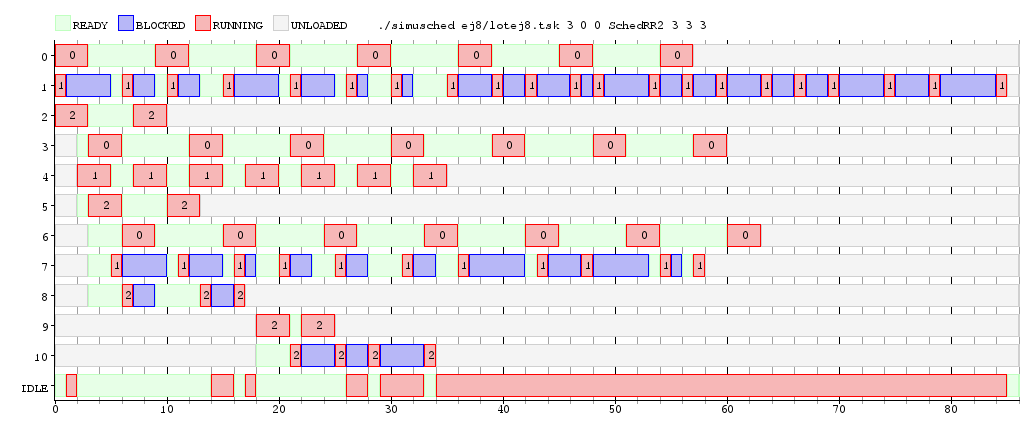
\includegraphics[width=\textwidth]{../ej8/rr2.png}
  \caption{}
\end{figure}

Se puede observar que no existe migración de núcleos, ya que todas las tareas mantienen su número de cpu a lo largo de toda la simulación.
En los instantes 0, 2 y 4 se ve que llegan las tareas y se les asignan los cores de la forma esperada. En el instante 4, los 3 cpu tienen 3 tareas cada uno. En el instante 15 el cpu 2 se queda sin tareas para ejecutar(la tarea 2 termina en el momento 2, la 5 en el 9 y la 13 en el 15). Por lo tanto se le asigna el IDLE_TASK por un ciclo de clock hasta que llegan dos nuevas tareas. Vemos que efectivamente se le asignan al core número 2, que es el que menos tareas tenía de los tres. 









